
\section{Resultaten}

\subsection{DV1: Beste classificatiemethode}
Het beste resultaat werd bereikt met Support Vector Machines gebruikmakend van \textit{stochastic gradient descent learning} en Elasticnet regularisatie. De woorden waren hierbij gestemd. De features waren zowel unigrams, bigrams als trigrams. Geen features zijn hierin weggelaten door minimale of maximale documentfrequenties. Het maximum aantal iteraties was 5 voor de grid search, maar alle resultaten zijn op basis van 100.\par
Tabel \ref{tab:classrapport} laat de scores zien per partij met het aantal documenten in de test set. De \textit{accuracy} voor deze classificatie is 0.80. De $F_1$ scores per partij liggen tussen de 0.7 en 0.9. De partijen met een sterke focus op één onderwerp, 50PLUS, PVV en PvdD, als ook de SGP hebben hoge scores, terwijl de coalitiepartijen, VVD en PvdA, lagere scores hebben. Figuur \ref{fig:confusionmatrix} laat zien waar de fouten in deze classificatie zitten. De meest karakteristieke features per partij zijn te zien in tabel \ref{tab:MostImportantWords}. Met meest karakteristiek worden de n-grams bedoeld die de hoogste coëfficiënt hebben in de classificatie en die dus relatief het meeste belangrijk zijn voor de classificatie van een partij. Hierin is te zien dat vrijwel alle n-grams achternamen van Kamerleden of partijnamen bevatten.\par

\begin{table}[H]
\caption{Classificatie scores per partij van beste classificatiemethode (SVM). Gemiddelde van vijf splitsingen van training en test set. Maximum aantal iteraties is 100.}
\label{tab:classrapport}
\centering
\begin{tabular}{lrrrlr}
\toprule
{} &  Precision &  Recall &  F1\_score & Accuracy &  Documenten \\
\midrule
50PLUS       &       0.97 &    0.85 &      0.91 &        - &        71.4 \\
CDA          &       0.80 &    0.79 &      0.80 &        - &       379.6 \\
ChristenUnie &       0.83 &    0.76 &      0.79 &        - &       215.4 \\
D66          &       0.78 &    0.75 &      0.76 &        - &       381.8 \\
GroenLinks   &       0.89 &    0.73 &      0.80 &        - &       209.2 \\
PVV          &       0.82 &    0.88 &      0.85 &        - &       345.0 \\
PvdA         &       0.72 &    0.71 &      0.71 &        - &       377.4 \\
PvdD         &       0.86 &    0.87 &      0.86 &        - &        81.2 \\
SGP          &       0.87 &    0.84 &      0.86 &        - &       134.8 \\
SP           &       0.73 &    0.85 &      0.78 &        - &       453.2 \\
VVD          &       0.77 &    0.73 &      0.75 &        - &       331.0 \\
Totaal       &       0.79 &    0.79 &      0.79 &     0.79 &      2980.0 \\
\bottomrule
\end{tabular}

\end{table}


\begin{figure}[H]
  \centering
    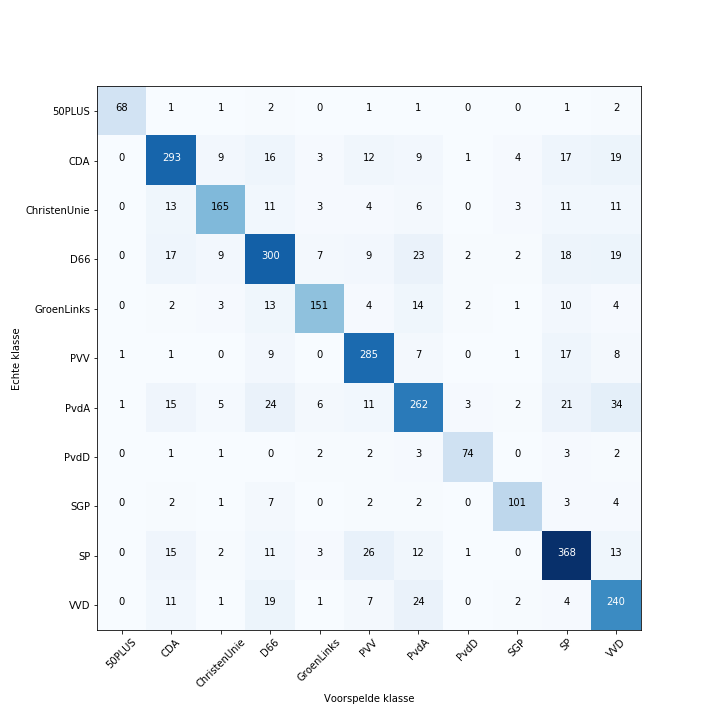
\includegraphics[width=0.50\paperwidth]{Verslag/Tables/confusionmatrix.png}
\caption{Confusion matrix van beste classificatiemethode (SVM). Gemiddelde van vijf splitsingen van training en test set.}
\label{fig:confusionmatrix}
\end{figure}



\begin{table}[H]
\caption{Meest karakteristieke n-grams per partij op basis van beste classificatie gedurende kabinet-Rutte II. N-grams die niet achternamen van Kamerleden of partijnamen bevatten, zijn dikgedrukt. }
\label{tab:MostImportantWords} 
\centering
\hspace*{-1in}
\begin{tabular}{lllll}
\toprule
          50PLUS &               CDA &         ChristenUnie &                  D66 &          GroenLinks \\
\midrule
          50plus &               cda &      de christenunie &                  d66 &          groenlinks \\
   lid krol naar &           het cda &         christenunie &         mijn fractie &    lid van tongeren \\
    het lid krol &            de cda &        lid dik faber &  leden van veldhoven &   lid voortman naar \\
        lid krol &       cda fractie &          het lid dik &       lid van meenen &    het lid voortman \\
   krol naar mij &    de cda fractie &              lid dik &        van veldhoven &        lid voortman \\
       krol naar &       lid omtzigt &            dik faber &            veldhoven &            voortman \\
            krol &   het lid omtzigt &                faber &    lid van veldhoven &            tongeren \\
      van 50plus &  lid omtzigt naar &     leden voordewind &         leden schouw &        van tongeren \\
 gepensioneerden &      omtzigt naar &  de leden voordewind &      de leden schouw &  leden van tongeren \\
         ouderen &  omtzigt naar mij &                  dik &               d66 is &   de leden voortman \\
\bottomrule
\end{tabular}
 
\end{table} 
\addtocounter{table}{-1} 
\begin{table}[H]
\caption{Meest karakteristieke n-grams per partij op basis van beste classificatie gedurende kabinet-Rutte II. N-grams die niet achternamen van Kamerleden of partijnamen bevatten, zijn dikgedrukt.  \emph{(Vervolg)}} 
\centering
\hspace*{-1.3in}
\begin{tabular}{llllll}
\toprule
              PVV &             PvdA &              PvdD &              SGP &             SP &             VVD \\
\midrule
              pvv &          de pvda &      lid ouwehand &              sgp &             sp &          de vvd \\
           de pvv &             pvda &  lid ouwehand nar &           de sgp &          de sp &             vvd \\
      islamitisch &    de partij van &  het lid ouwehand &      sgp fractie &   lid van gerv &  de vvd fractie \\
        lid graus &    van de arbeid &      ouwehand nar &   de sgp fractie &     sp fractie &     vvd fractie \\
    het lid graus &        de arbeid &  ouwehand nar mij &     led dijkgraf &  de sp fractie &       de vvd is \\
    lid graus nar &    partij van de &          ouwehand &  de led dijkgraf &   van gerv nar &          vvd is \\
          miljard &       partij van &       vor de dier &      led van der &       gerv nar &      vor de vvd \\
    graus nar mij &     pvda fractie &           de dier &  de led bisschop &   gerv nar mij &      wat de vvd \\
        graus nar &           arbeid &              dier &     led bisschop &           gerv &     vvd betreft \\
 madlener nar mij &  de pvda fractie &     de partij vor &           sgp is &       van gerv &  de vvd betreft \\
\bottomrule
\end{tabular}
 
\end{table}

\subsection{DV2: Invloed van namen}
In tabel \ref{tab:MostImportantWords} was al te zien dat de meest karakteristieke n-grams voornamelijk achternamen van Kamerleden of partijnamen bevatten. In tabel \ref{tab:rapportonlynames} zijn de scores te zien voor een classificatie met alleen achternamen van Kamerleden en partijnamen. De \textit{accuracy} is 0.61. De scores zijn gedaald ten opzichte van de resultaten van deelvraag 1, maar ruim hoger dan de baseline scores.\par
\begin{table}[H]
\caption{Classificatierapport van beste classificatie met alleen achternamen van Kamerleden en partijnamen. Hiervoor is alleen gebruikgemaakt van unigrams. Gemiddelde van vijf splitsingen van training en test set.}
\label{tab:rapportonlynames}
\centering
\begin{tabular}{lrrr}
\toprule
{} &  Precisie &  Sensitiviteit &  $F_1$ score \\
\midrule
50PLUS       &       0.82 &    0.88 &      0.85\\
PvdD         &       0.68 &    0.78 &      0.69 \\
GroenLinks   &       0.71 &    0.66 &      0.68  \\
PVV          &       0.66 &    0.71 &      0.67  \\
CDA          &       0.67 &    0.65 &      0.66  \\
ChristenUnie &       0.66 &    0.58 &      0.62 \\
SP           &       0.61 &    0.64 &      0.62  \\
VVD          &       0.68 &    0.57 &      0.62  \\
SGP          &       0.69 &    0.54 &      0.60  \\
D66          &       0.56 &    0.53 &      0.54  \\
PvdA         &       0.56 &    0.51 &      0.52  \\
\midrule
Totaal       &       0.64 &    0.62 &      0.62  \\
\bottomrule
\end{tabular}

\end{table}

In tabel \ref{tab:rapportwithoutnames} zijn de $F_1$scores te zien van classificatie met achternamen van Kamerleden en partijnamen vervangen. De \textit{accuracy} hiervan is 0.58. De scores zijn aanzienlijk lager dan die uit deelvraag 1 en ook nog lager dan van de classificatie met alleen namen. Wel zijn de scores nog ruim hoger dan de baseline. In tabel \ref{tab:MostImportantWordsWithoutNames} is vervolgens te zien welke n-grams het meest karakteristiek zijn per partij voor deze classificatie.\par
\begin{table}[H]
\caption{Classificatie scores per partij van beste classificatie zonder achternamen van Kamerleden en partijnamen met het relatieve verschil ten opzichte van tabel \ref{tab:classrapport}. Gemiddelde van vijf splitsingen van training en test set.}
\label{tab:rapportwithoutnames}
\centering
\begin{tabular}{lcccc}
\toprule
{} &  Precision &  Recall &  $F_1$ score &  $\Delta F_1$ score (\%) \\
\midrule
SGP          &       0.71 &    0.73 &      0.72 & -18 \\
PvdD         &       0.75 &    0.70 &      0.72 & -19 \\
PVV          &       0.63 &    0.80 &      0.70 & -19 \\
ChristenUnie &       0.68 &    0.46 &      0.55 & -21 \\
CDA          &       0.52 &    0.53 &      0.52 & -23 \\
SP           &       0.54 &    0.71 &      0.61 & -24 \\
D66          &       0.55 &    0.55 &      0.55 & -28 \\
VVD          &       0.54 &    0.49 &      0.52 & -30 \\
50PLUS       &       0.86 &    0.49 &      0.62 & -32 \\
PvdA         &       0.51 &    0.48 &      0.50 & -32 \\
GroenLinks   &       0.64 &    0.38 &      0.48 & -41 \\
\midrule
Totaal       &       0.59 &    0.58 &      0.57 &        -29 \\
\bottomrule
\end{tabular}

\end{table}

\begin{table}[H] 
\caption{Meest karakteristieke n-grams per partij op basis van classificatie uit deelvraag 1 zonder achternamen van Kamerleden en partijnamen gedurende kabinet-Rutte II.} 
\label{tab:MostImportantWordsWithoutNames} 
\centering
\hspace*{-0.8in}
\begin{tabular}{lllll}
\toprule
                 50PLUS &             CDA &   ChristenUnie &           D66 &              GroenLinks \\
\midrule
        gepensioneerden &  PARTIJ fractie &   mensenhandel &  mijn fractie &                     zou \\
                ouderen &        inwoners &         zullen &          mijn &       kamer hierover te \\
                 oudere &          PARTIJ &       gezinnen &       fractie &     belastingontwijking \\
 koopkrachtontwikkeling &        regering &      inderdaad &    natuurlijk &            in elk geval \\
               plussers &             wij &  vluchtelingen &   het kabinet &        persoonsgebonden \\
                     50 &     de regering &       kinderen &    belangrijk &               elk geval \\
              werkenden &            hier &           hoop &       vandaag &                  in elk \\
            50 plussers &            echt &          motie &        kansen &  hierover te informeren \\
   voor gepensioneerden &         fractie &     onder meer &       kabinet &          schone energie \\
            overwegende &              de &     constateer &  buitengewoon &             hierover te \\
\bottomrule
\end{tabular}
 
\end{table} 
\addtocounter{table}{-1} 
\begin{table}[H] 
\caption{Meest relevante n-grams per partij op basis van classificatie uit deelvraag 1 zonder achternamen van Kamerleden en partijnamen gedurende kabinet-Rutte II. \emph{(Vervolg)}} 
\centering
\hspace*{-1.3in}
\begin{tabular}{llllll}
\toprule
         PVV &             PvdA &              PvdD &                    SGP &            SP &            VVD \\
\midrule
 islamitisch &      mijn partij &              dier &               dank zer &       huurder &     volgen mij \\
       islam &       leerkracht &            de bio &  mevrouw de voorzitter &    segregatie &        liberal \\
     miljard &           tevred &     bio industrie &             mevrouw de &      herindel &      speelveld \\
    de islam &        circulair &               bio &           eenverdiener &        armoed &     verzekerar \\
 asielzoeker &   open standaard &        aan de bio &               allerlei &     de bevolk &          aruba \\
     brussel &          gezamen &  de bio industrie &                   punt &       jazeker &     ondernemer \\
   nederland &       ieder kind &            milieu &                 nadruk &          zegt &       regelgev \\
       grenz &  duurzam energie &     dierenwelzijn &                  woord &  bureaucratie &       aangegev \\
  immigratie &               en &          de natur &                 vanuit &     tenderned &  PARTIJNAAM is \\
          al &       lager over &   klimaatverander &                    oog &  ouderbijdrag &     essentieel \\
\bottomrule
\end{tabular}
 
\end{table}



\subsection{DV3: Oppositie of regering}
In figuur \ref{fig:distributies} zijn de distributies van de errors, zoals gedefinieerd in formule \ref{eq:error} te zien van combinaties van regerings- en oppositiepartijen.
\begin{figure}[H]
    \centering
    \hspace*{-0.2in}
    \subfloat[Tussen twee regeringspartijen (N=200)]{{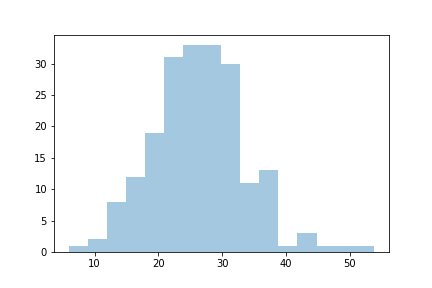
\includegraphics[width=7cm]{Verslag/Handmatig/Regering.png} }}%
    \subfloat[Tussen twee oppositiepartijen (N=8100)]{{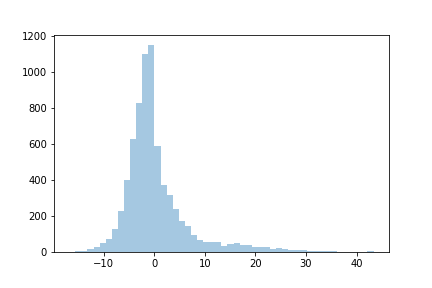
\includegraphics[width=7cm]{Verslag/Handmatig/Oppositie.png} }}\quad
    \hspace*{-0.2in}
    \subfloat[Tussen een regeringspartij en een oppositiepartij (N=4000)]{{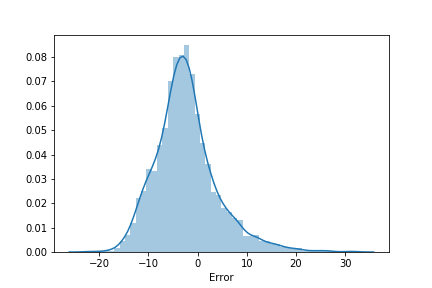
\includegraphics[width=7cm]{Verslag/Handmatig/Mix.png} }}%
    \subfloat[Totaal (N=12100)]{{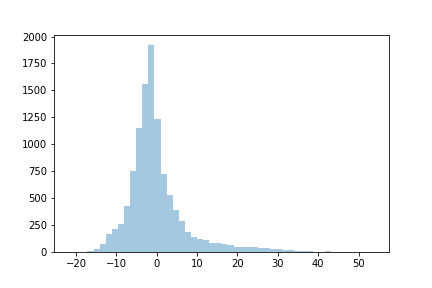
\includegraphics[width=7cm]{Verslag/Handmatig/Totaal.png} }}\quad
    \caption{Genormaliseerde distributie van de error uit formule \ref{eq:error} voor de verschillende combinaties.}%
    \label{fig:distributies}%
\end{figure}
Voor alle distributies kan de nulhypothese verworpen worden dat deze normaal verdeeld zijn, hoewel dit wel verwacht was. In tabel \ref{tab:whitney} is vervolgens te zien dat er een significant verschil is tussen de distributies binnen regering en oppositie tegenover de distributie tussen regering en oppositiepartij.

\begin{table}[H]
\caption{Uitslagen van eenzijdige Mann-whitneytoets tussen de distributie tussen een regeringspartij en oppositiepartij en twee distributies. $\alpha$ is 0.05.}
\label{tab:whitney}
\centering
\begin{tabular}{lrr}
\toprule
{} &  p-waarde &  U-waarde\\
\midrule
Tussen twee regeringspartijen       &       \num{7.04e-124} &    717042 \\
Tussen twee oppositiepartijen         &       \num{4.4e-108} &    16328471 \\
\bottomrule
\end{tabular}
\end{table}
In tabel \ref{tab:WoordenBalkenende4} zijn de meest karakteristieke n-grams te zien voor classificatie van kabinet-Balkenende IV. Hierin zijn geen opvallende overlappen te zien van regeringspartijen met de classificatie van kabinet-Rutte II in tabel \ref{tab:MostImportantWordsWithoutNames}.
\begin{table}[H] 
\caption{Meest karakteristieke n-grams per partij op basis van classificatie uit deelvraag 2 gedurende kabinet-Balkenende IV.} 
\label{tab:WoordenBalkenende4} 
\centering
\hspace*{-0.6in}
\begin{tabular}{lllll}
\toprule
                  CDA &        ChristenUnie &              D66 &          GroenLinks &         PVV \\
\midrule
       PARTIJ fractie &  fractie van PARTIJ &          premier &       PARTIJfractie &     burgers \\
                  wij &      de fractie van &       de premier &  fractie van PARTIJ &        onze \\
              fractie &          de fractie &          ik hoop &          de fractie &        niet \\
           wij hebben &         fractie van &     arbeidsmarkt &      de fractie van &        deze \\
             KAMERLID &        mijn fractie &  de arbeidsmarkt &         fractie van &  immigratie \\
                 dank &             geweest &             hoop &           politieke &  natuurlijk \\
 PARTIJ fractie heeft &              moment &              hij &             premier &     politie \\
          zorgvuldige &             termijn &   schone energie &                deal &  de burgers \\
                  ons &       verschillende &          plannen &                  ik &      burger \\
         buitengewoon &       beantwoording &           kunnen &                  en &        door \\
\bottomrule
\end{tabular}
 
\end{table} 
\addtocounter{table}{-1} 
\begin{table}[H] 
\caption{Meest karakteristieke n-grams per partij op basis van classificatie uit deelvraag 2 gedurende kabinet-Balkenende IV.\emph{(Vervolg)}} 
\centering
\hspace*{-0.4in}
\begin{tabular}{lllll}
\toprule
         PvdA &              PvdD &                    SGP &            SP &             VVD \\
\midrule
          wij &            dieren &           mijn fractie &          zegt &          PARTIJ \\
   belangrijk &     dierenwelzijn &          beantwoording &    leerlingen &    onze fractie \\
      vrouwen &     bio industrie &                    wel &        mensen &  PARTIJ fractie \\
         alle &            natuur &          de voorzitter &            is &         fractie \\
          ben &  de bio industrie &       de voorzitter ik &          niet &              je \\
  volgens mij &            de bio &             natuurlijk &       vandaar &     ondernemers \\
           of &               bio &                diverse &  bureaucratie &            awbz \\
 mijn collega &       dierproeven &               allerlei &            nu &           markt \\
   antwoorden &       veehouderij &      voorzitter ik wil &   voorstellen &          praten \\
         punt &         industrie &  mevrouw de voorzitter &       leraren &      timmermans \\
\bottomrule
\end{tabular}
 
\end{table}
In tabel \ref{RegeringOppositie} zijn de resultaten van de classificatiescores te zien waarbij de classificatie getraind is op een zittingsperiode, maar getest op een andere. De resultaten zijn sterk  gedaald, maar nog boven de baseline. De daling verschilt enorm per partij en zittingsperiode met dalingen van $F_1$ scores tussen 12 en 92\%. \par
\begin{table}[H]
\caption{$F_1$ scores van de classificatie getraind op ene zittingsperiode en getest op andere zittingsperiode. Scores van een classificatie getraind en getest op kabinet-Rutte II zonder 50PLUS zijn bijgevoegd ter referentie, als ook de relatieve daling. De classificatiemethode uit deelvraag 1 is gebruikt zonder achternamen van Kamerleden en partijnamen. Partijen met een asterisk zijn gewisseld van partij-status.}
\centering
\hspace*{-0.2in}
\label{RegeringOppositie}
\begin{tabular}{ll|cccc}
\toprule
{}& {}&\multicolumn{4}{l}{Training set$\rightarrow$ Test set}\\
\midrule
{} &Rutte II &\multicolumn{2}{l}{\makecell{Balkenende IV $\rightarrow$ Rutte II\\Baseline = 0.11}}&  \multicolumn{2}{l}{\makecell{Rutte II $\rightarrow$ Balkenende IV\\Baseline = 0.12}}  \\
{} & $F_1$ & $F_1$ & $\Delta F_1$ score (\%) &  $F_1$& $\Delta F_1$ score (\%) \\
\midrule
SGP          &0.74&       0.56 &  -24 &   0.49 & -34 \\
PvdD         &0.73&       0.64 &  -12 &  0.45 & -38\\
PVV          &0.70&       0.50 &  -29 &   0.60  & -14 \\
SP           &0.61&       0.41 & -33 &   0.53 & -13 \\
ChristenUnie* &0.55&       0.37 &  -33 & 0.22 &-60 \\
D66          &0.54&       0.16 &  -70 & 0.28 & -48 \\
CDA*          &0.53&       0.28 & -47&   0.43 & -19 \\
PvdA         &0.52&       0.29 & -44 &   0.27 & -48 \\
VVD*          &0.51&       0.18 & -65 &   0.10 & -80  \\ 
GroenLinks   &0.49&       0.31 &  -37 &   0.04 & -92 \\ \hline
Totaal       &0.58&       0.34 & -41 &  0.35 & -40 \\
\bottomrule
\end{tabular}

\end{table}


\subsection{DV4: Links/rechts}
\begin{figure}[H]
  \centering
    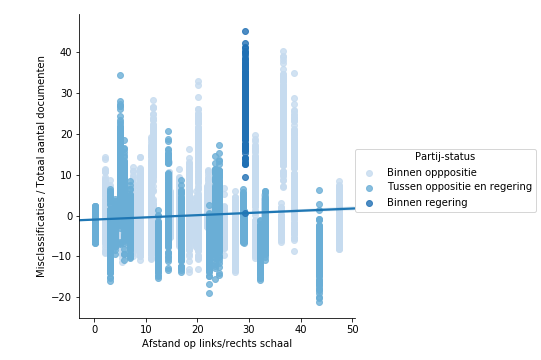
\includegraphics[width=0.60\paperwidth]{Verslag/Tables/Ideology.png}
\caption{Aantal misclassificaties gedeeld door totaal aantal documenten per spreker tegenover totaal aantal documenten van een spreker. Misclassificaties zijn totaal van 5-fold cross-validation, waardoor documenten vaker mee kunnen tellen. De pearson correlatie is -0.28 en de p-waarde \num{1.07e-4}.}
\label{fig:misclassifiedsprekers}
\end{figure}

\subsection{DV5: Woordgebruik van sprekers}
In tabel \ref{tab:rapporttaalgebruik} staan de scores van classificatie waarbij de Kamerleden verdeeld zijn over de training en test set. De scores zijn hierbij amper hoger dan de baseline.
\begin{table}[H]
\caption{Classificatierapport van beste classificatie met de Kamerleden verdeeld over training en test set. Gemiddelde van vijf splitsingen van training en test set.}
\label{tab:rapporttaalgebruik}
\centering
\begin{tabular}{lrrrr}
\toprule
{} &  Precisie &  Sensitiviteit &  $F_1$ score &  $\Delta F_1$ score (\%) \\
\midrule
50PLUS       &       0.29 &    0.06 &      0.09 &           \\
CDA          &       0.12 &    0.20 &      0.14 &          \\
ChristenUnie &       0.08 &    0.14 &      0.09 &           \\
D66          &       0.22 &    0.22 &      0.22 &          \\
GroenLinks   &       0.16 &    0.04 &      0.05 &          \\
PVV          &       0.29 &    0.50 &      0.37 &          \\
PvdA         &       0.25 &    0.19 &      0.21 &          \\
PvdD         &       0.46 &    0.17 &      0.22 &          \\
SGP          &       0.17 &    0.05 &      0.07 &           \\
SP           &       0.34 &    0.33 &      0.33 &          \\
VVD          &       0.31 &    0.26 &      0.24 &          \\
\midrule
Totaal       &       0.31 &    0.24 &      0.24 &         \\
\bottomrule
\end{tabular}

\end{table}

